\begin{comment}
\documentclass[a4paper,11pt]{book}
\usepackage[T1]{fontenc}
\usepackage[utf8]{inputenc}
\usepackage[a4paper,top=4.0cm,bottom=4.5cm,left=3.5cm,right=3.5cm,
bindingoffset=0mm]{geometry}
%\usepackage[italian]{babel}
\usepackage[english]{babel}
\usepackage{amsmath}
\usepackage{graphics}
\usepackage{graphicx}
\usepackage{textcomp}
\usepackage{array}
\usepackage{tabularx}
\usepackage{booktabs}
\usepackage{multicol}
\usepackage{listings}
\lstset{language=C++,
basicstyle=\small\ttfamily,
showstringspaces=false,
numbers=left,
numberstyle=\tiny,
breaklines=true,
columns=fullflexible}
\usepackage{hyperref}
\usepackage{amsmath}
\usepackage{amssymb}
\usepackage{fancyhdr}
\pagestyle{fancy}
\usepackage{acronym}
\usepackage{comment}
\lhead{}
\rhead{\small \slshape \leftmark}

\newenvironment{citazione}
{\begin{quotation}\small}
{\end{quotation}}
\begin{document}
\end{comment}

\chapter*{Introduzione}
Il Modello Standard è una teoria fisica elegante e compatta che descrive le interazioni fondamentali tra le particelle.
Fino a questo momento, il suo successo nel riprodurre i dati sperimentali è impressionante e copre diversi
ordini di grandezza di energia. Al fine di spiegare l'origine delle masse per le particelle osservate, il Modello Standard introduce 
nella sua formulazione matematica un campo fisico aggiuntivo, il cui quanto è costituito dal bosone di Higgs. Grazie a questo grado di libertà aggiuntivo, la massa (nuda)
delle particelle può essere realizzata tramite gli accoppiamenti dei loro campi al campo del bosone di Higgs. La massa nuda di una particella viene successivamente
rinormalizzata a seguito delle correzioni quantistiche fino al valore della sua massa fisica (cioè quella che si misura negli esperimenti) e
anche la massa stessa del bosone di Higgs riceve correzioni quantistiche nella teoria del Modello Standard. In particolare, tra queste
è presente un correzione a loop\footnote{Un loop è una struttura chiusa in un diagramma di Feynman} dovuta al contributo del quark top,
che presenta una divergenza di tipo quadratico.
\newline
Per sopperire a tale problema, negli ultimi decenni sono state formulate
diverse teorie oltre il Modello Standard (\acs{BSM}) che prevedono l'esistenza di particelle pesanti aggiuntive che 
permetterebbero di cancellare il contributo divergente proveniente dal quark top.
\newline
In particolare, molte teorie (\textit{Little Higgs}, \textit{extra-dimensions}, \textit{composite Higgs}) richiedono la presenza
di nuovi quark tipo up, che in questa tesi saranno indicati genericamente come quark $T$.
Tali quark aggiuntivi sono, di fatto, repliche pesanti del quark top, ma presentano accoppiamenti di tipo vettoriale al bosone di Higgs.
\newline
In questo lavoro di tesi verranno presentati i risultati della prima analisi di ricerca di repliche vettoriali del quark top, con la
presenza di un bosone di Higgs ricostruito nello stato finale. L'analisi è stata effettuata sui dati raccolti durante tutto
il 2012 dall'esperimento CMS corrispondenti a una luminosità integrata di $19.6 ~fb^{-1}$ e prendendo in considerazione lo scenario
\acs{BSM} definito dal \textit{branching ratio} di decadimento $B.R.(T\rightarrow tH)=1$.
\newline
In assenza di un significativo eccesso rispetto alle previsioni nell'ipotesi di solo fondo, si è proceduto a fissare limiti di esclusione al
95 \% di livello di confidenza sulla sezione d'urto del processo di segnale.
\newline
Nel Capitolo 1 verrà descritta la fisica del Modello Standard e le sue principali limitazioni teoriche, che hanno portato alla formulazione
di teorie fisiche ulteriori.
\newline
Nel Capitolo 2 sarà descritto l'esperimento \acs{CMS} nel suo insieme, con particolare riguardo al calorimetro elettromagnetico \acs{ECAL}.
\newline
Nel Capitolo 3 saranno descritte le tecniche di ricostruzione degli oggetti fisici, presenti nello stato finale dell'analisi.
\newline
Nel Capitolo 4 verrà descritta la strategia di definizione della selezione degli eventi impiegata in quest'analisi. 
\newline
Nei Capitoli 5 e 6 saranno presentati i risultati di tale analisi e tratte le conclusioni.



\chapter{Modello Standard: descrizione, limitazioni e possibili estensioni}
In questo capitolo sarà introdotto sinteticamente il Modello Standard delle particelle elementari.
Si passerà quindi a esporre le principali limitazioni della teoria e a presentarne alcune possibili estensioni,
allo scopo di superare tali limitazioni.
\section{Standard Model: quadro generale}
Il Modello Standard, in inglese \ac{SM}, è una delle teorie scientifiche meglio verificate dello scorso secolo e costituisce, attualmente, 
il modello di riferimento comunemente accettato per la descrizione delle interazioni delle particelle elementari.

\medskip
Il Modello Standard è un modello matematico che permette di modellizzare le particelle elementari come quanti di campi fisici.
Nella sua formulazione, il Modello Standard include solo tre delle quattro forze fondamentali della Natura: la forza forte, la
forza elettromagnetica e la forza debole. Non include invece, nel suo quadro, la forza gravitazionale.
\newline
Le descrizione del Modello Standard organizza le particelle di materia ordinaria, fermioni di spin $\frac{1}{2}$, in 
tre famiglie di leptoni e tre famiglie di quark (ognuna ripetuta in tre colori) e prevede l'
esistenza di particelle elementari di spin 1 mediatrici delle interazioni.
In aggiunta, il Modello Standard richiede la presenza di una ulteriore particella di spin $0$:
il bosone di Higgs. %(Le particelle elementari del Modello Standard sono mostrate in fig. \ref{particles}).
\begin{figure}[!htbp]
\begin{center}
\includegraphics[scale=0.55]{Immagini/simplemodel2}
\end{center}
\caption[Particelle elementari del Modello Standard]{La figura mostra le particelle elementari del Modello Standard divise 
in particelle ordinarie (fermioni) e mediatori di forza 
(bosoni di Gauge). I fermioni, a loro volta, sono divisi in quark e leptoni. La forza forte influenza solo i quark, dal momento che
i leptoni sono privi del numero quantico di colore, che detta gli accoppiamenti a questa forza. Sia i quark che i leptoni sono divisi in
tre generazioni di doppietti. Tutte le masse delle particelle sono realizzate tramite l'interazione con il campo del bosone di Higgs}
\label{particles}
\end{figure}

All'interno del Modello Standard, il punto di partenza di tutti i calcoli è costituito dalla Lagrangiana, per mezzo
della quale, imponendo il \textit{Principio di Minima Azione}, possono essere ricavate le equazioni del moto della teoria.
\newline
La Lagrangiana del Modello Standard è invariante sotto il gruppo di simmetria $SU(3)_{c}\times SU(2)_{L}\times U(1)_{Y}$, in cui è notevole
il fatto che la forza elettromagnetica, la forza debole e la forza forte, nonostante le loro manifestazioni profondamente diverse su scala
macroscopica, possano essere tutte descritte nello stesso quadro matematico delle teorie di gauge.
\newline
In particolare, la forza forte è associata al gruppo di simmetria 
$SU(3)_{c}$, mentre la forza elettromagnetica e la forza debole sono associate, a corte distanze,
allo stesso gruppo di simmetria $SU(2)_{L}\times U(1)_{Y}$.

\medskip
La descrizione matematica della forza forte è realizzata dal gruppo $SU(3)_{c}$ dove il pedice sta per \textit{colore}, un 
numero quantico aggiuntivo, introdotto da Han and Nambu \cite{nambu} nel 1965 per evitare il paradosso apparente che il modello a quark
sembrava richiedere una violazione del principio di esclusione di Pauli, molto ben verificato fino a quel momento.

\medskip
La formulazione completa della forza forte in termini di una teoria di gauge quantizzata risale invece al 1973 ad 
opera di Fritzsh \cite{Fritzsh},
Gross e Wilczec \cite{Gross}, Weinberg \cite{Weinberg}.

\medskip
Dal momento che tutte le particelle osservate negli esperimenti ai collisori adronici sono prive del numero quantico di colore (a differenza dei quark che sono colorati), deve
esistere un meccanismo, tra il processo elementare e l'effettiva rivelazione delle particelle nello stato finale, che porti dai quark
liberi colorati (prodotti nell'interazione elementare) alle particelle osservate, prive di colore.
\newline
Questo meccanismo, non ancora del tutto compreso dal punto di vista teorico, è noto come \textit{adronizzazione} e implica che la produzione dei quark nella collisione sia rivelata attraverso getti
di particelle, ossia strutture a cono con elevata attività adronica all'interno. Il processo di formazione dei getti dipende dalla scala della QCD, nota come $\Lambda_{QCD}$, rispetto all'impulso del
partone colorato dello stato finale del processo elementare. Tale scala $\Lambda_{QCD}$ rappresenta la soglia che discrimina 
il regime perturbativo della teoria (quello in cui è applicabile la teoria delle perturbazioni e il formalismo dei diagrammi
di Feynman) da quello non perturbativo. Per la proprietà della QCD nota come \textit{libertà asintotica} la teoria perturbativa risulta applicabile
se la scala di energia del processo elementare $\sqrt{\hat{s}}\gg\Lambda_{QCD}$. La formazione dei getti ha inizio dal partone del processo elementare, 
tramite processi di emissione di gluoni e conseguente
conversione di questi in coppie quark-antiquark. A ogni emissione/conversione l'energia posseduta dai partoni al termine della 
catena diminuisce e, di conseguenza, ad un certo punto verrà raggiunto il regime non perturbativo, dove i calcoli espliciti non
possono più essere portati avanti.
La formazione dei getti, pertanto, avviene soltanto se la scala di energia del partone iniziale da cui ha origine il processo
di adronizzazione, il suo impulso trasverso risulta $p_{T}\gg\Lambda_{QCD}$.

\bigskip
Il gruppo $SU(2)_{L}\times U(1)_{Y}$ descrive la parte elettrodebole del modello e rappresenta l'unificazione teorica, realizzata ad opera
di Glashow, Weinberg e Salam \cite{salam}, delle forze elettromagnetica e debole.
In tale teoria, dall’imposizione di una simmetria di gauge locale $SU(2)_{L}\times U(1)_{Y}$ in ogni punto dello spazio-tempo 
quadri-dimensionale, emerge la presenza di quattro bosoni vettori, tre per il gruppo $SU(2)$ ($W_i ~,i=1,2,3$) e uno per il
gruppo $U(1)$ ($B_{\mu}$).

I campi fisici
vengono ottenuti tramite combinazione lineare di questi ultimi e sono:
\begin{center}
 $A_{\mu}=\sin(\theta)W_{\mu}^{3}+\cos(\theta)B_{\mu}$
\end{center}
\begin{center}
 $Z_{\mu}=\cos(\theta)W_{\mu}^{3} -\sin(\theta)B_{\mu}$
\end{center}
\begin{center}
 $W_{\mu}^{\pm}=\dfrac{W_{\mu}^{1}\mp W^{2}_{\mu}}{\sqrt{2}}$
\end{center}

dove $\theta$ è l'angolo di Weinberg (angolo di interazione debole), $A^{\mu}$ rappresenta il campo del fotone, $W^{\pm}$
sono i campi dei bosoni fisici carichi e $Z$ è il campo del bosone neutro.

\medskip
Dato che solo la forza elettromagnetica è sperimentata come una forza a lunga distanza, questo implica che il resto della simmetria elettrodebole
è nascosta a lunga distanza (bassa energia). Nel Modello Standard questo viene spiegato tramite un meccasismo di rottura spontanea della simmetria elettrodebole da parte del vuoto.
Il Modello Standard formula tale meccanismo di rottura spontanea, in inglese \ac{EWSB}, in termini di un solo
nuovo grado di libertà: il bosone di Higgs. Questa, dunque, costituisce la ragione fondamentale della sua introduzione nel quadro della teoria
\cite{rottura}.

\medskip
Grazie all'introduzione del bosone di Higgs nella formulazione attuale del Modello Standard
la simmetria elettrodebole è rotta spontaneamente dal vuoto. La teoria così completata porta a previsioni fino a questo momento 
in accordo con tutti i dati raccolti e a tutte le scale di energia esplorate.

\medskip
Nella prossima sezione sarà descritto e formulato matematicamente il ruolo del bosone di Higgs nel meccanismo di rottura spontanea
della simmetria, così come previsto nel Modello Standard.

\section{Il ruolo del bosone di Higgs nella rottura spontanea di simmetria}
Il principio fondamentale che guida la costruzione della Lagrangiana del Modello Standard è la richiesta di invarianza sotto una simmetria locale
(di \textit{gauge}).
Ciò semplicemente impedisce la possibilità di aggiungere alcun termine di massa nella Lagrangiana perché violerebbe tale principio di invarianza,
ma al contempo è in disaccordo con ogni evidenza sperimentale.
\newline
La soluzione, nel quadro del Modello Standard, è fornita tramite l'introduzione di una particella scalare neutra, nota appunto come bosone di Higgs.

\medskip
Per introdurre il concetto di rottura spontanea di simmetria, si consideri una generica Lagrangiana invariante sotto una certa trasformazione
di simmetria.
Un determinato autostato di tale Lagrangiana può essere degenere oppure no: se è non degenere esso è invariante sotto la stessa simmetria di
cui gode la Lagrangiana; se invece è degenere (cioè non è l'unico autostato che corrisponde a un determinato autovalore dell'operatore) può non
seguire la simmetria della Lagrangiana.
\newline
Nel caso in cui sia lo stato fondamentale ad essere degenere non esiste una scelta univoca per descrivere lo stato di minima energia e la scelta
di un particolare stato invece di un altro rende possibile il meccanismo di rottura spontanea della simmetria. 
Un meccanismo analogo si verifica già in modelli di fisica dello stato solido come i superconduttori.
\newline
Nel Modello Standard la rottura spontanea di simmetria viene resa possibile nella sua forma più elementare grazie all'introduzione
, avvenuta ad opera di Brout, Englert e Higgs nel 1964 (\cite{rottura},\cite{higgs2}), di un campo scalare neutro $\phi$, il campo di Higgs.
\newline
Al nuovo campo è associata la seguente Lagrangiana:
\begin{equation}
 L_{Higgs}=(D_{\mu}\phi)^{\dagger}D^{\mu}\phi -V(\phi)
\end{equation}
dove $D_{\mu}$ rappresenta l'operatore di derivata covariante e il potenziale $V(\phi)$ è:
\begin{equation}
 V(\phi)=\mu^{2}\phi^{\dagger}\phi+\lambda(\phi^{\dagger}\phi)^{2}
\end{equation}
Per avere una teoria stabile il minimo valore ammesso dell'energia deve essere finito. Ciò implica che l'autovalore minimo dell'operatore
Hamiltoniano deve essere finito.
Dato che la Lagrangiana $L_{Higgs}$ entra, cambiata di segno, nell'Hamiltoniano, ciò implica uteriormente che il potenziale $V(\phi)$ deve essere limitato
inferiormente.
Imponendo un $\mu^{2}<0$ il minimo del potenziale sarebbe finito ma degenere.
Tale caso è mostrato in figura \ref{minimo}, dove appare chiaro che tutti gli infiniti minimi di un potenziale di questo tipo ricadrebbero su una
circonferenza attorno al massimo locale del potenziale, posizionato nell'origine.
\begin{figure}[!htbp]
\begin{center}
\includegraphics[scale=0.5]{Immagini/minimo}
\end{center}
\caption{Il potenziale $V(\phi)$ del campo di Higgs}
\label{minimo}
\end{figure}

\`{E} noto da richieste generali di coerenza interna (teorema asintotico) che il vuoto di una generica teoria (cioè lo stato di minima energia)
deve sempre essere unico. Perciò, se si ammette un potenziale $V(\phi)$ con $\mu^{2}<0$ lo si dovrà ulteriormente completare con un ulteriore
termine del tipo $\epsilon\phi^{\dagger}+\epsilon^{*}\phi$, che solo in un secondo momento sarà annullato richiedendo il limite 
$\epsilon\rightarrow0$.
\newline
Il potenziale sarà quindi modificato secondo:
\begin{equation}
  V(\phi)=\mu^{2}\phi^{\dagger}+\lambda(\phi^{\dagger}\phi)^{2}+\epsilon\phi^{\dagger}+\epsilon^{*}\phi
\end{equation}

In questo modo, l'ambiguità della degenerazione del punto di minimo viene risolta dal termine aggiuntivo (detto \textit{driving term}) che
seleziona un minimo specifico tra gli infiniti possibili.
Attorno al minimo $\eta$ si possono pertanto studiare le piccole oscillazioni del campo $\phi$ che, attorno a tale configurazione
e nella particolare scelta della \textit{gauge unitaria},
si può esprimere come:
\begin{equation}
 \phi=\eta+\dfrac{\sigma(x)}{\sqrt{2}}
\end{equation}

Sviluppando la Lagrangiana del Modello Standard attorno al minimo $\eta$ emergono termini quadratici nei campi di materia, che corrispondono ai termini di massa
delle varie particelle.

\medskip
Inoltre, descrivendo i campi di materia in termini di componenti di chiralità è possibile conferire massa ai fermioni, tramite
termini di interazione alla Yukawa. Infatti accoppiando un doppietto levogiro e un singoletto destrogiro con il campo di Higgs si può
scrivere la Lagrangiana di massa dei quark come:
\begin{equation}
 L_{qH}=\sum_{ij}g_{ij}^{D}\bar{Q}\phi D_{j}+g_{ij}^{U}\epsilon_{ab}\bar{U}Q^{a}_{j}\phi^{b}+h.c.
\end{equation}

dove $Q_{i}$ rappresenta il generico doppietto sinistrorso e $U_{i}$ e $D_{i}$ sono i campi destrogiri di tipo \textit{up} e \textit{down};
$g_{ij}^{D}$ e $g_{ij}^{U}$ sono le costanti di accoppiamento dei campi fermionici con il campo di Higgs.
Sostituendo il valore del campo di Higgs attorno al minimo e diagonalizzando si ottiene la Lagrangiana di massa nella sua forma diagonale:
\begin{equation}
 L_{qm}=\bar{D}_{ph}m_{d}D_{ph}+\bar{U}_{ph}m_{u}U_{ph}
\end{equation}
dove $m_{u,d}$ sono matrici diagonali e $D_{ph}$ e $U_{ph}$ sono i campi fisici dei quark, cioè gli autostati di massa della teoria.
Tali autostati di massa risultano differenti dagli autostati delle interazioni deboli e legati a questi ultimi tramite la relazione:
\begin{equation}
 D_{ph}=U^{\dag}_{CKM}D
\end{equation}
\begin{center}
 $U=U_{ph}$
\end{center}

Il disallineamento tra i due insieme di autostati è realizzato tramite i coefficienti della matrice $U_{CKM}$, esprimibile in generale come:
\begin{equation}
\begin{bmatrix} V_{ud} & V_{us} & V_{ub} \\ V_{cd} & V_{cs} & V_{cb} \\ V_{td} & V_{ts} & V_{tb} \end{bmatrix}
\end{equation}

dove gli elementi non diagonali permettono il decadimento (debole) tra famiglie diverse di quark.


\medskip
\`{E} bene anche ricordare che non tutte le particelle del Modello Standard hanno massa (ad esempio il fotone è rigorosamente a massa nulla), 
pertanto lo stato fondamentale che viene selezionato tramite il driving term deve sì rompere la simmetria elettrodebole $SU(2)\times U(1)$ ma
conservare la simmetria di carica elettrica $U(1)$.

\subsection{Proprietà fisiche del bosone di Higgs}\label{prop_higgs}
Il meccanismo di generazione delle masse può essere esteso a tutte le particelle massive del Modello Standard ed è, in sintesi, dovuto
all'accoppiamento del campo di Higgs con i campi di materia e intrinsicemante legato alla rottura spontanea di simmetria per quanto concerne l'accoppiamento ai bosoni di gauge.
Data la presenza di questi termini di Lagrangiana il bosone di Higgs godrà di diversi
meccanismi di produzione (che nel caso del collisore adronico LHC sono riportati in figura \ref{higgs_prod}) e potrà quindi decadere in diversi canali di decadimento, i cui rapporti di decadimento, detti \textit{branching ratios} (B.R.),
sono riportati in figura \ref{branch_rat} in funzione della massa dell'Higgs.
\newline
Il Modello Standard non fissa alcuna massa per il bosone di Higgs, come pure per tutte le altre particelle previste. Di conseguenza, 
in passato tutte le ricerche sono state effettuate nel più ampio spettro di massa possibile.

\begin{figure}[!htbp]
\begin{center}
\includegraphics[scale=0.3]{Immagini/higgs_prod.png}
\end{center}
\caption[Sezioni d'urto dei meccanismi di produzione del bosone di Higgs]{Sezioni d'urto dei meccanismi di produzione del 
bosone di Higgs per un'energia del centro di massa $\sqrt{s}=8 ~TeV$}
\label{higgs_prod}
\end{figure}

\begin{figure}[!htbp]
\begin{center}
\includegraphics[scale=0.4]{Immagini/branch_rat.png}
\end{center}
\caption{Branching Ratios dei canali di decadimento del bosone di Higgs}
\label{branch_rat}
\end{figure}

Come si vede in figura \ref{branch_rat_lm}, per un bosone di Higgs di massa attorno a $125 ~GeV$, il canale di decadimento più probabile è $b\bar{b}$, 
ma la insufficiente risoluzione sperimentale nella massa invariante di 2 getti e l'elevata sezione d'urto per il fondo di produzione di 2 getti originati da quark $b$ rende questo
canale difficile da utilizzare sperimentalmente come canale di scoperta. 
Lo stesso discorso si può applicare al decedimento $H\rightarrow\tau\tau$.
I canali di decadimento con bosoni vettori sono i più interessanti per la scoperta di un Higgs del Modello Standard,
in particolare il decadimento $H\rightarrow ZZ$ con decadimento dei bosoni $Z$ in elettroni o muoni e il canale di decadimento $H\rightarrow\gamma\gamma$.
Tali canali, infatti, permettono la ricostruzione completa della cinematica di decadimento e, di conseguenza, la misura della massa dell'Higgs.


Data l'importanza che riveste in questa analisi, è bene fornire ulteriori dettagli circa il decadimento del bosone di Higgs 
in due fotoni.
\newline
Per un Higgs di massa $\le 140 ~GeV$, questo canale è un canale di notevole importanza (ed è stato anche uno dei canali fondamentali per la sua scoperta).
Nonostante il suo B.R. relativamente basso rispetto ad altri canali (figura \ref{branch_rat_lm}), gode di uno stato finale particolarmente pulito data la presenza di soli
due fotoni isolati rispetto al resto dell'attività adronica, per la cui rivelazione gli esperimenti del CERN, ATLAS e CMS (\ref{CMS_sec}),  sono ottimizzati.

\begin{figure}[!htbp]
\begin{center}
\includegraphics[scale=0.4]{Immagini/branch_rat_lm.png}
\end{center}
\caption{Branching Ratios dei canali di decadimento del bosone di Higgs per basse masse}
\label{branch_rat_lm}
\end{figure}

Dato che i fotoni non hanno massa, non esiste un termine di Lagrangiana diretto che accoppi i fotoni al bosone di Higgs, 
di conseguenza, tale decadimento avverrà per mediazione di una particella massiva e carica, per cui quindi esiste un vertice di tipo
elettromagnetico che la accoppi al fotone.
L'ordine più basso di tale decadimento è perciò almeno a un loop (e ciò rende ragione del suo B.R. basso), secondo i diagrammi di Feynman 
riportati in fig. \ref{hgg}.

\begin{figure}[!htbp]
\begin{center}
\includegraphics[scale=0.8]{Immagini/higgsdecays1.png}
\end{center}
\begin{center}
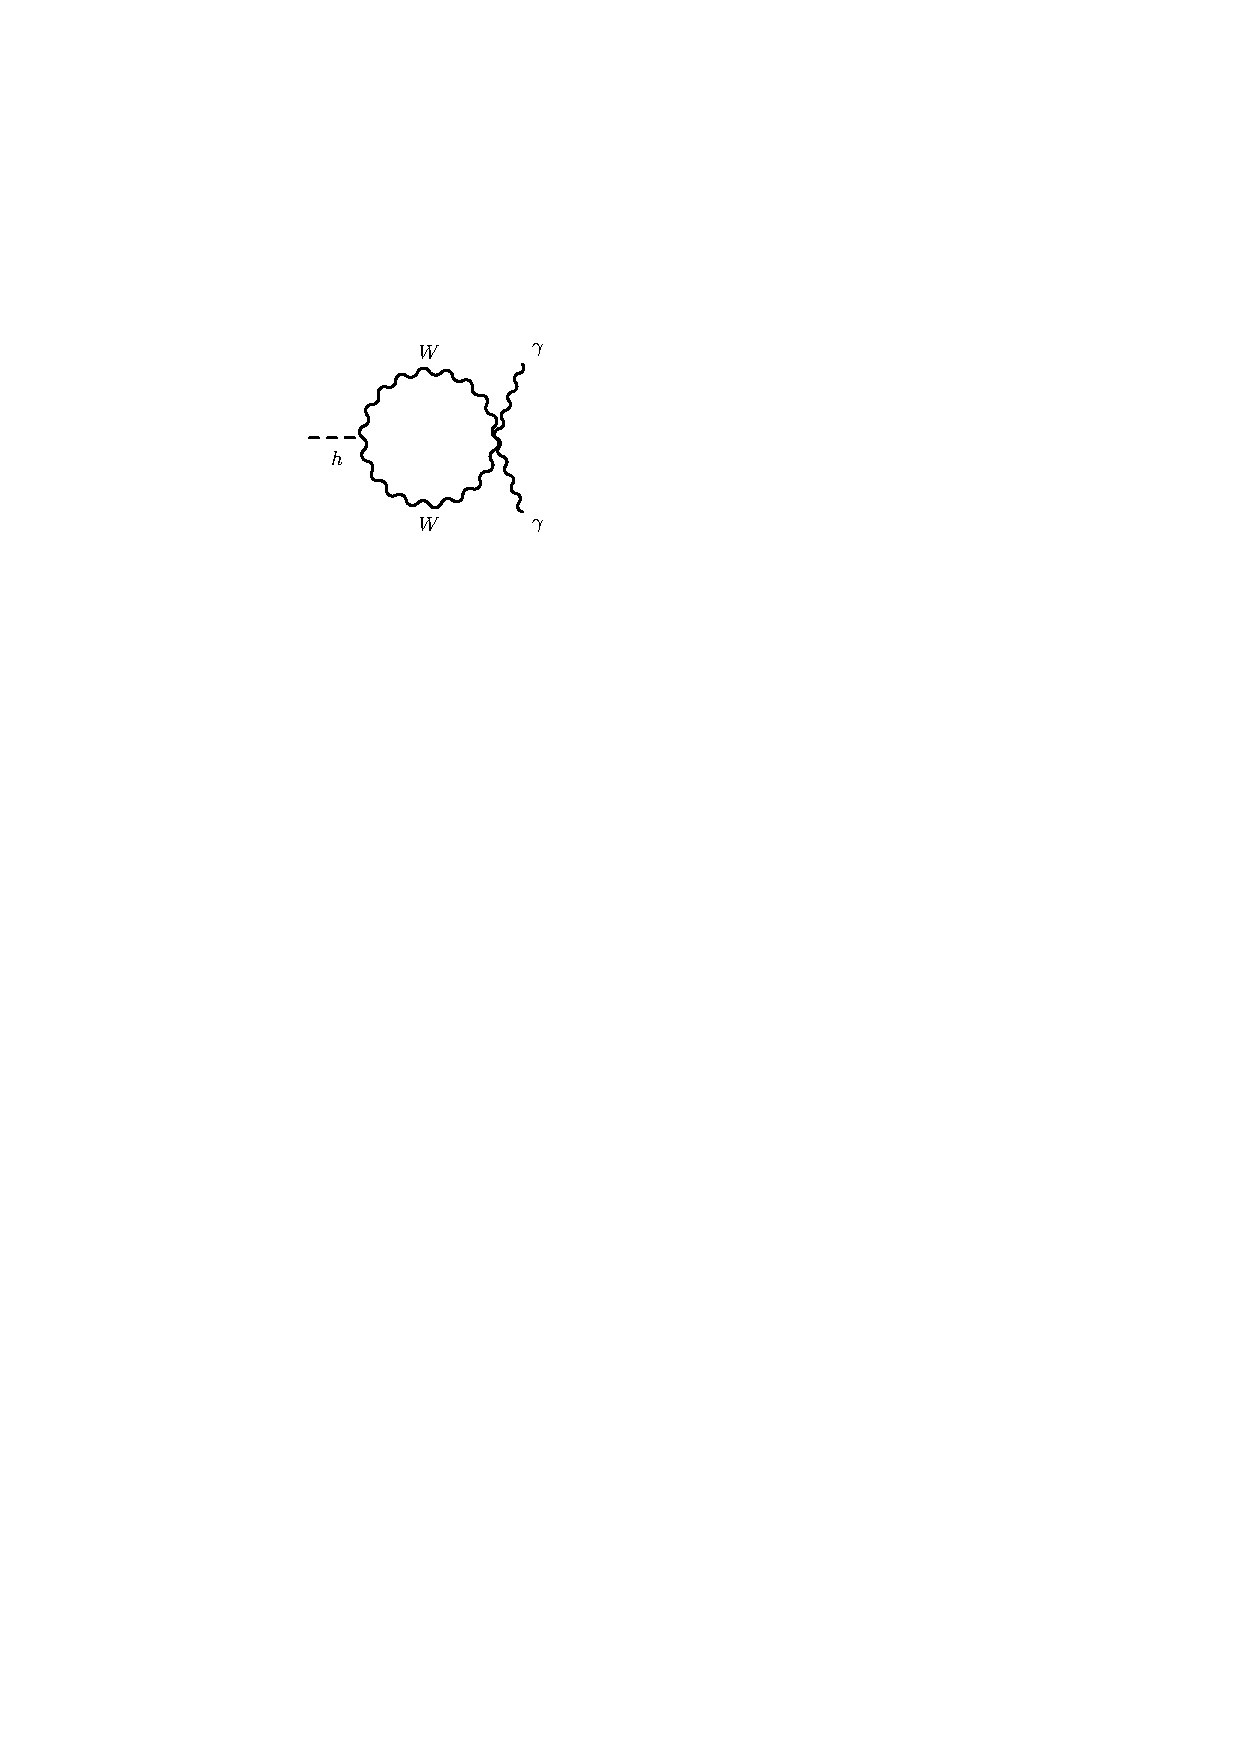
\includegraphics[scale=0.9]{Immagini/hgg.pdf}
\end{center}
\caption[Decadimento $h\rightarrow\gamma\gamma$]{Principali meccanismi di decadimento del bosone di Higgs ($h$) in due fotoni}
\label{hgg}
\end{figure}

La larghezza di decadimento del processo $H\rightarrow\gamma\gamma$ si ottiene esplicitamente in teoria delle perturbazioni:
\begin{equation}\label{Hgg}
 \Gamma(H\rightarrow\gamma\gamma)\sim\dfrac{G_{F}\alpha_{em}^{2}M^{3}_H}{128\pi^{3}\sqrt{2}}|7-\frac{16}{9}+\cdots|^{2}
\end{equation}
dove $G_F$ è la costante di Fermi, $\alpha_{em}$ è la costante di struttura fine. Dalla formula \ref{Hgg} risulta che i termini 
associati al loop del $W$ (+7) e del top (-16/9) hanno segno opposto.
 
Di conseguenza il B.R. di decadimento risulta:
\begin{equation}
 B.R.(H\rightarrow\gamma\gamma)= 2.28\times 10^{-3}
\end{equation}
\begin{center}
 $m_{H}=125 ~GeV$
\end{center}

\section{Misura delle proprietà fisiche del bosone di Higgs}
\medskip
La scoperta di una nuova risonanza compatibile con il bosone di Higgs previsto dal Modello Standard, effettuata al \ac{CERN} dai due esperimenti
ATLAS \cite{atlasHiggs} e CMS \cite{cmsHiggs} e annunciata nel Luglio 2012,
costituisce certamente uno dei maggiori risultati nelle ricerche della moderna fisica delle particelle.
\newline
Tuttavia, non è ancora confermato che la nuova risonanza sia \textit{il} bosone di Higgs previsto dal Modello Standard.
A tal fine è necessario testare
una per una le proprietà della nuova risonanza e stabilire se soddisfino o meno le previsioni della teoria.
\newline
In particolare, a fissata massa del bosone di Higgs, i suoi accoppiamenti agli altri campi di materia sono fissati a loro volta
dal valore delle masse fisiche delle particelle, note ormai con elevata precisione.
\newline 
Il metodo di ricerca consiste quindi nello stabilire se la nuova risonanza di massa:
\begin{center}
 $m_{H}=125.5 \pm 0.2 ~(stat) ^{+0.5}_{-0.6} ~(sist) ~GeV$ \footnote{ATLAS, aggiornato MORIOND 2013 }
\end{center}
\begin{center}
$m_{H}=125.8 \pm 0.5 ~(stat) \pm 0.2 ~(sist) ~GeV$ \footnote{CMS, aggiornato MORIOND 2013}
\end{center}
abbia o meno gli accoppiamenti previsti dal Modello Standard e che, di conseguenza, decada secondo le modalità e i B.R. teorici.
\newline
La misura delle proprietà del bosone di Higgs può essere effettuata sia esaminando quantità inclusive, come il rapporto tra la sezione d'urto osservata, moltiplicata per il relativo rapporto di decadimento,
rispetto a quella prevista in un particolare canale di decadimento, sia verificando la compatibilità degli accoppiamenti
osservati con quelli previsti dal Modello Standard.


Gli strumenti statistici impiegati nel calcolo della quantità $\mu=\dfrac{\sigma}{\sigma_{SM}}$, in ascissa di fig.\ref{higgs_decay_meas},
saranno descritti in dettaglio in (\ref{limite superiore}).

\medskip
Si descriverà invece, in breve, la procedura eseguita per verificare la compatibilità degli accoppiamenti con quelli previsti dal 
Modello Standard \cite{coupl_check}.
\newline
In un approccio di analisi non basato su uno specifico modello BSM, i dati vengono interpretati nel contesto di una teoria effettiva, tramite una Lagrangiana
che compendia tutte le possibili deviazioni rispetto al Modello Standard.
Il primo passo, in tale approccio, consiste nello scrivere la Lagrangiana più generale possibile che sia inviarante, all'interno
del gruppo $SU(3)_{c}\times SU(2)_{L}\times U(1)_{Y}$, sotto trasformazioni di Lorentz e di gauge.
Tale Lagrangiana può essere, in maniera generale, espansa in operatori di dimensionalità via via crescente.

\begin{equation}
 \mathcal{L}_{eff}=\mathcal{L}_{SM}+\mathcal{L}_{d=5}+\mathcal{L}_{d=6}+\cdots
\end{equation}

dove $\mathcal{L}_{SM}$ è la Lagrangiana attuale del Modello Standard in presenza \textit{del} bosone di Higgs di tale modello;
$\mathcal{L}_{d=5}$ agisce sul settore della massa dei neutrini e risulta non rilevante per quanto concerne la misura
degli accoppiamenti del bosone di Higgs; $\mathcal{L}_{d=6}$ include, invece, operatori di dimensione 6 che modificano gli 
accoppiamenti dell'Higgs del Modello Standard; operatori di dimensionalità più alta non darebbero significative deviazioni sperimentalmente significative,
data la precisione raggiunta attualmente nelle misure. Una base conveniente nella quale esprimere tali operatori è fornita
in \cite{coupl_check_2}.

L'approccio completamente rigoroso sarebbe quello di considerare la Lagrangiana effettiva nella sua interezza. Tuttavia,
l'ammontare dei dati non è ancora sufficiente per considerare tutti i possibili operatori (e relativi parametri liberi)
di tale Lagrangiana. Di conseguenza
la Lagrangiana effettiva completa viene semplificata, ignorando gli operatori che porterebbero a
deviazioni, rispetto alle predizioni del Modello Standard, o già escluse in maniera sufficientemente stringente (anche se non
definitiva) dalle precedenti misure o non accessibili con la quantità di dati attualmente disponibile (è il caso, ad esempio,
di alcuni operatori presenti in $\mathcal{L}_{d=6}$ che porterebbero
ad una violazione di CP non misurabile).
\newline
La Lagrangiana effettiva semplificata appare, nei termini che coinvolgono gli accoppiamenti al bosone di Higgs come:

\begin{equation}
\begin{split}
 \mathcal{L}_{h,sim}&=\dfrac{h}{v}\Bigl( 2c_v m^2_W W^+_\mu W^{-\mu} ~+ ~c_v m^2_Z Z_\mu Z^{\mu}\\&~- ~c_u\sum_{q=u,c,t}m_q \bar{q}q ~- ~c_d
 \sum_{q=d,s,b}m_q \bar{q}q ~- ~c_l\sum_{l=e,\mu,\tau}m_l \bar{l}l\\& ~+ ~\dfrac{1}{4}c_{gg}G^{a}_{\mu\nu}G^{a\mu\nu} ~- ~\dfrac{1}{4}
 c_{\gamma\gamma}\gamma_{\mu\nu}\gamma^{\mu\nu} ~- ~\dfrac{1}{2}c_{WW}W^{+}_{\mu\nu}W^{-\mu\nu} \\&~- ~\dfrac{1}{4}c_{ZZ}Z_{\mu\nu}Z^{\mu\nu}
 ~- ~\dfrac{1}{2}c_{Z\gamma}\gamma_{\mu\nu}Z^{\mu\nu}\Bigr)
 \end{split}
\end{equation}
dove $h$ è il campo di Higgs, $v$ il suo valore di aspettazione sul vuoto.
La Lagrangiana efficace semplificata $\mathcal{L}_{h,sim}$ dipende da 7 parametri liberi (esistono infatti 2 vincoli che
i 9 coefficienti $c$ devono verificare).

La Lagrangiana del settore di Higgs del Modello Standard è riottenuta nel limite:
\begin{center}
 $c_v=c_u=c_d=c_l=1 ~; ~c_{gg}=c_{\gamma\gamma}=c_{Z\gamma}=0$
\end{center}

Al fine di stabilire il valore dei parametri $c$ è possibile esprimere tali coefficienti in termini di osservabili fisici, quali
larghezze di decadimento e sezioni d'urto di produzione.
\newline
Ad esempio, per il processo $H\rightarrow b\bar{b}$, il rapporto tra la larghezza di decadimento osservata e quella prevista dal Modello Standard si può esprimere:
\begin{center}
 $\dfrac{\Gamma_{bb}}{\Gamma_{bb}^{SM}}\simeq c^{2}_{d}$
\end{center}

oppure, per il processo $H\rightarrow\gamma\gamma$:
\begin{center}
 $\dfrac{\Gamma_{\gamma\gamma}}{\Gamma^{SM}_{\gamma\gamma}}\simeq\dfrac{|\hat{c}_{\gamma\gamma}|^{2}}{|
 \hat{c}_{\gamma\gamma,SM}|^2}$
 \end{center}
\begin{center}
 $\hat{c}_{\gamma\gamma}=c_{\gamma\gamma}+10^{-2}[0.97c_v - 0.21c_u +\cdots]$
\end{center}
\begin{center}
 $|\hat{c}_{\gamma\gamma,SM}|\simeq0.0076$
\end{center}

e così di seguito.

Combinando le misure attuali di LHC nei differenti canali, è possibile eseguire delle procedure di fit
sui dati sperimentali ottenendo, dalla minimizzazione del valore del $\chi^{2}$ di tale fit, la stima più recente dei 7 coefficienti\footnote{Aggiornata 23/07/2013} 
\cite{falk}.
\newline
Tale stima riporta i seguenti valori:
\begin{center}
 $c_v=1.04^{+0.03}_{-0.03}$
\end{center}
\begin{center}
 $c_u=0.55^{+0.66}_{-1.72}$
\end{center}
\begin{center}
 $c_d=1.03^{+0.26}_{-0.20}$
\end{center}
\begin{center}
 $c_l=1.04^{+0.21}_{-0.21}$
\end{center}
\begin{center}
 $c_{gg}=0.005^{+0.022}_{-0.031}$
\end{center}
\begin{center}
 $c_{\gamma\gamma}=0.0001^{+0.0018}_{-0.0021}$
\end{center}
\begin{center}
 $c_{Z\gamma}=0.006^{+0.015}_{-0.028}$
\end{center}

tutti compatibili, entro gli errori al 68\% di livello di confidenza, con quelli attesi per il Modello Standard.

\begin{figure}[!htbp]
\begin{center}
\includegraphics[scale=0.4]{Immagini/higgs_decay_cms.png}
\end{center}
\begin{center}
\includegraphics[scale=0.2]{Immagini/higgs_decay_atlas.png}
\end{center}
\caption{Combinazione dei risultati sperimentali divisi per canale di decadimento dell'Higgs}
\label{higgs_decay_meas}
\end{figure}

Ad oggi, inoltre, anche i risultati (fig. \ref{higgs_decay_meas}) delle misure della quantità $\dfrac{\sigma}{\sigma_{SM}}$ sia di ATLAS che di CMS confermano la compatibilità della nuova risonanza con il bosone di Higgs 
del Modello Standard, con una precisione intorno al 20-30\% nei rapporti di decadimento.

\medskip
Tuttavia, benché non ci siano motivi di natura sperimentale per mettere in dubbio la completezza del Modello Standard,
esiste almeno una motivazione di carattere più generale e astratto: il cosiddetto \textit{problema della gerarchia}.


\section{Il problema della gerarchia}
Dopo la scoperta, realizzata da ATLAS \cite{atlasHiggs} e CMS \cite{cmsHiggs}, di una nuova risonanza compatibile con il bosone di Higgs , 
la sua massa, come riportato esplicitamente sopra, è già nota con notevole precisione.
Dai risultati sperimentali risulta pertanto che il bosone di Higgs presenti una massa confrontabile con la massa dei bosoni W e Z, quindi confrontabile con la scala di rottura della simmetria 
elettrodebole dell'ordine $O(100 ~GeV)$.
\newline
Come tutte le altre particelle della teoria, anche la massa del bosone di Higgs riceve correzioni radiative che, tramite il 
processo di rinormalizzazione (si veda più avanti), portano il valore della sua massa cosiddetta nuda, cioè ricavata dal propagatore quantistico all'ordine più
basso in teoria delle perturbazioni, al valore della sua massa fisica di circa 125 GeV.

\begin{figure}[!htbp]
\begin{center}
\includegraphics[scale=0.5]{Immagini/higgs_new_loop}
\end{center}
\caption{In figura sono mostrati i contributi divergenti più significativi alla massa del bosone di Higgs, previsti dal Modello Standard }
\label{higgs_loop}
\end{figure}

Tuttavia, la massa di un campo scalare elementare (come appunto è il bosone di Higgs nel Modello Standard) riceve correzioni quadratiche
divergenti. Ciò, in assenza di un qualche nuovo tipo di protezione derivante da una nuova simmetria, rende apparentemente poco probabile
la natura dell'Higgs come bosone leggero, dal momento che l'esistenza di correzioni quadratiche dell'ordine della scala di validità della teoria
richiederebbe cancellazioni di precisione estrema per lasciare la massa dell'Higgs ad un valore dell'ordine di 100 GeV.
\newline
Questo problema va sotto il nome di problema della gerarchia o della naturalezza, ed è una delle principali considerazioni 
che potrebbero suggerire l'esistenza di possibili sceneri \acs{BSM}.

\medskip
Senza scopo di completezza, verrà brevemente descritto il processo di rinormalizzazione e quindi la natura del problema della gerarchia.
\newline
Il processo di rinormalizzazione corregge la massa nuda (al quadrato) del bosone di Higgs con un termine aggiuntivo $\delta m^{2}_{H}$

\begin{equation}
\label{hier}
 m^{2}_{Hnuda}=m^{2}_{Hrin}+\delta m^{2}_{H}
\end{equation}

\bigskip
Dato che il Modello Standard non include la gravità, non può essere la teoria fisica definitiva.
\newline
Ciò detto, in linea di principio, la sua formulazione potrebbe però essere valida fino alla scala di Planck $M_{P} \approx 10^{19} ~GeV$ 
dove gli effetti quantistici legati alla forza gravitazionale non sono più trascurabili.
\newline
Se ciò fosse vero, l'unico motivo di ragionamento sarebbe come mai esiste una gerarchia così ampia (17 ordini di grandezza)
tra la massa dei bosoni intermedi $M_{W}$ e la scala di Planck $M_{P}$.
\newline
Risulta che le correzioni alla massa dell'Higgs sono quadratiche nella scala di validità $\Lambda$ della teoria.
Se lo Standard Model fosse valido fino alla scala di Planck ($\Lambda=M_P$), il termine correttivo $\delta m^{2}_{H}$ nell'equazione \ref{hier} 
dovrebbe essere circa $\delta m^{2}_{H}\approx M^{2}_{P}$. Tale è infatti la scala di energia alla quale, 
in linea di principio, potrebbero giungere le particelle virtuali presenti nei diagrammi di correzione radiativa alla massa dell'Higgs.
\newline
Perciò per ottenere il risultato sperimentale $m^{2}_{Hrin}=(125 ~GeV)^{2}$ è necessario che si verifichi:
\begin{equation}
 m^{2}_{Hnuda} -M^{2}_{P}\approx (125 ~GeV)^{2}
\end{equation}
o, equivalentemente, dividendo per $M^{2}_{P}$
\begin{equation}
 \dfrac{m^{2}_{Hnuda}}{M^{2}_{P}} -1\approx \dfrac{(125 ~GeV)^{2}}{M^{2}_{P}}
\end{equation}

Il membro destro dell'equazione è dell'ordine di $(125 ~GeV/M_{P})^{2} \approx 10^{-34}$.
\newline
Ciò porta alla seguente relazione, abbastanza poco naturale:
\begin{equation}
 \dfrac{m^{2}_{Hnuda}}{M^{2}_{P}}=1+10^{-34}
\end{equation}

che implica, in sostanza, una cancellazione dei due termini con una precisione molto alta 
(questo problema è anche noto come \textit{fine tuning}).

\medskip
Il problema può essere mitigato abbassando la scala di validità del Modello Standard fino a una certa scala $\Lambda < M_P$.

\medskip
Per esempio, si prenda: $\Lambda=10 ~TeV$.

\medskip
Oltre questa scala non è più noto come calcolare i diagrammi a loop.
\newline
Grazie all'introduzione della scala $\Lambda$ è facile mostrare che il problema della gerarchia nasce
semplicemente perché i contributi correttivi alla massa dell'Higgs sono (quadraticamente) divergenti, nel Modello Standard.
Per $\Lambda=10 ~TeV$, le correzioni sono \cite{higgs_corr}:

\begin{center}
 top $\approx -(2 ~TeV)^{2}$

 bosoni di Gauge $\approx (0.7 ~TeV)^{2}$

Higgs $\approx (0.5 ~TeV)^{2}$
\end{center}

Queste correzioni richiedono una cancellazione a livello di una parte su cento.
Infatti, riadattando l'equazione \ref{hier}:
\begin{equation}
 m^{2}_{Hnuda}=m^{2}_{Hrin}-(2 ~TeV)^{2}+(0.7 ~TeV)^{2}+(0.5 ~TeV)^{2}
\end{equation}

\medskip
Applicando alcune semplici approssimazioni:
\begin{equation}
 m^{2}_{Hnuda}=m^{2}_{Hrin} -(100 ~GeV\times20)^{2}+(100 ~GeV\times7)^{2}+(100 ~GeV\times5)^{2}
\end{equation}
\begin{equation}
\label{hier_2}
 m^{2}_{Hnuda}=m^{2}_{Hrin} +(100 ~GeV)^{2}(-400+50+25)
\end{equation}
In questo caso, dunque, il termine $\delta m^{2}_{H}$ nell' eq. \ref{hier} è $\approx -325\times(100 ~GeV)^{2}$
\newline
Dividendo per $\delta m^{2}_{H}$ nell' eq. \ref{hier_2}:
\begin{equation}
\label{hier_3}
 \dfrac{m^{2}_{Hnuda}}{\delta m^{2}_{H}}\approx 1-10^{-2}
\end{equation}

Quindi, sotto l'assunzione di una scala $\Lambda=10 ~TeV$, cioè che esista nuova fisica a questa scala di energia,
si richiede un fine tuning di (solo) una parte su 100.
\newline
Di conseguenza, il problema della gerarchia può essere mitigato semplicemente abbassando la scala di validità del Modello Standard
dalla scala di Planck alla scala effettiva $\Lambda=10 ~TeV$.
D'altra parte, se la scala di nuova fisica attesa è 
$\Lambda = 1 ~TeV$, la necessità del fine-tuning scompare completamente
(sarebbe richiesta una precisione nella cancellazione dei termini di circa 1 parte su 10).
\newline
A questa scala di energia ci si aspetta di trovare evidenza di nuove particelle, la cui esistenza dovrebbe essere
dettata da nuove simmetrie, che cancellerebbero in maniera naturale i contributi divergenti alla massa dell'Higgs,
provenienti, in particolare, dal quark top.
\newline
Dato che i contributi divergenti dovuti ai bosoni di Gauge e all'Higgs stesso nei loop sono più piccoli,
le nuove particelle che li cancellerebbero possono essere ancora più pesanti: circa $5 ~TeV$ per nuovi
bosoni di Gauge, e circa $10 ~TeV$ per una nuova particella di tipo Higgs.

\medskip
In sintesi, quindi, il problema della gerarchia emerge dal fatto che il bosone di Higgs ha una massa molto inferiore alla scala
di Planck.
\newline
Questo semplice fatto, apparentemente, implica un fine tuning molto spinto (che appare non naturale) tra le correzioni radiative 
e la massa nuda dell'Higgs.

In linea di principio, una qualsiasi teoria potrebbe essere consistente anche in presenza di fine tuning.
Tuttavia, una teoria che non lo richieda, risulterebbe essere più naturale e, in definitiva, più elegante. 

\section{Possibili soluzioni al problema della gerarchia}
Esistono due principali paradigmi di soluzioni al problema della gerarchia (anche noto come problema della naturalezza):
classi di teorie supersimmetriche e teorie non supersimmetriche che richiedono la presenza di nuovi fermioni aggiuntivi rispetto
a quelli previsti dal Modello Standard.\footnote{Una ulteriore soluzione alternativa al problema della gerarchia è data da teorie con dimensioni 
spaziali aggiuntive. Tali teorie sono guidate dal principio che l'apparente debolezza della forza gravitazionale sia 
il risultato della propagazione dei campi gravitazionali in un volume spaziale molto più ampio dato dalle dimensioni
aggiuntive, nelle quali ai soli campi 
gravitazionali è consentito propagarsi. In questo caso, quindi, la scala di Planck risulta molto più 
grande della scala elettrodebole solo nello spazio a 4 dimensioni dove sono relegati i campi di materia del Modello Standard.}

\medskip
L'esempio più celebre di protezione per la massa di un Higgs leggero è dato dalla supersimmetria che prevede l'esistenza di una 
simmetria tra bosoni e fermioni e prevede, quindi, per ogni particella del Modello Standard un partner supersimmetrico dallo spin intero/semi-intero 
a seconda che si tratti di un fermione o di un bosone.
Secondo tale modello, il contributo divergente delle correzioni radiative associate a ogni campo del Modello Standard è
cancellato da quello dell'equivalente partner supersimmetrico, con opposta statistica di spin.
\newline
In particolare, il contributo del quark top sarebbe parzialmente bilanciato dal contributo del suo partner scalare, 
il cosiddetto \textit{stop} (lo \textit{stop} in molte teorie supersimmetriche è quindi lo squark più leggero).
Lo stesso meccanismo regola tutti gli altri contributi divergenti alla massa dell'Higgs. Dopo la rinormalizzazione, restano dei contributi 
logaritmicamente divergenti, dovuti alla rottura della supersimmetria, che rendono meno stringente il fine tuning.
\newline
In questo lavoro di tesi, non saranno considerate tali classi di teorie supersimmetriche.

\medskip
Un'altra possibile soluzione al problema della gerarchia richiede, in generale, pur non ricorrendo alla supersimmetria,  partner fermionici
del quark top con masse non di molto superiori ai $500 ~GeV$.
In questo tipo di teorie, le correzioni radiative alla massa dell'Higgs dovute al quark top sono bilanciate dal contributo dei nuovi 
partner fermionici dello stesso spin del quark top, ma con accoppiamenti di tipo vettoriale.
\newline
Negli ultimi trent'anni sono stati introdotti numerosi modelli fisici di questo tipo, con lo scopo di risolvere il problema della gerarchia.
Essi sono però raggruppabili in tre diverse classi di modelli, ognuno con le sue particolarità: modelli che prevedono dimensioni fisiche
aggiuntive (noti genericamente come \textit{extra dimensions-models} \cite{extra} e a cui si è già accennato), modelli che introducono una nuova 
dinamica forte che porta
a un bosone di Higgs composto (\textit{composite Higgs} (\cite{strong1},\cite{strong2}) e teorie in cui il bosone di Higgs 
è uno pseudo-bosone di Goldstone di una simmetria
globale rotta spontaneamente (teorie \textit{little Higgs} (\cite{little1}-\cite{little3}).
Le ultime due classi di modelli sono abbastanza simili concettualmente tra loro: in particolare, nei modelli \textit{little Higgs}
la massa dell'Higgs è protetta dalle divergenze quadratiche dall'esistenza di una simmetria globale (approssimata), 
dalla cui rottura spontanea emerge il bosone di Higgs come relativo bosone di Nambu-Goldstone (e quindi a massa nulla,
per il teorema di Goldstone). La massa fisica del bosone di Goldstone emerge, in questi modelli, dalla
rottura esplicita della simmetria globale nella Lagrangiana. Affinché tale rottura esplicita non sia troppo severa vengono
introdotti campi aggiuntivi nella teoria (tra cui campi di partner del quark top). 
\newline
I modelli di Higgs composto, invece,
traggono origine dall'osservazione che, nella QCD, esistono campi scalari leggeri (pioni, kaoni) senza che emergano problemi di naturalezza.
Ciò è dovuto al fatto che tali stati non sono elementari ma composti.
Assumendo, pertanto, l'esistenza un nuovo settore di interazioni forti è possibile interpretare il bosone di Higgs quale (quasi)
bosone di Goldstone della nuova simmetria rotta spontaneamente e perciò, nel limite di simmetria esatta, rigorosamente a massa 
nulla.
\newline
A partire da queste classi generali, i singoli modelli teorici possono essere implementati in numerosi modi specifici.
\`{E} pertanto cruciale individuare le segnature sperimentali comuni ai vari modelli al fine di indirizzare
le linee di ricerca nella maniera più generale possibile.

\medskip
I nuovi fermioni previsti devono avere natura di tipo vettoriale (ciòè entrambe le componenti di chiralità devono trasformare nello stesso
modo all'interno del gruppo di simmetria $SU(2)\times U(1)$) perché, in caso contrario, si sarebbero già dovuti vedere degli effetti
nel principale meccanismo di produzione dell'Higgs al \ac{LHC}: la fusione di gluoni (Si veda fig. \ref{gluon_fusion}).

\begin{figure}[!htbp]
\begin{center}
\includegraphics[scale=0.25]{Immagini/gluon_fusion}
\end{center}
\caption{Diagramma di Feynman del principale meccanismo di produzione dell'Higgs: la fusione di gluoni \label{gluon_fusion}}
\label{pair_T}
\end{figure}

Il contributo dominante all'interno del loop è portato dalla particella più pesante presente nel modello, dal momento che
gli accoppiamenti con il bosone di Higgs crescono all'aumentare della massa delle particelle.
\newline
Ciò implica che, nel Modello Standard, il contributo più importante è dovuto al quark top. Nel caso, invece, esistessero nuovi fermioni
di quarta generazione, cioè semplici repliche a più alta massa di quelli del Modello Standard, il loro contributo nel loop dovrebbe
essere già visibile sperimentalmente, in particolare aumentando considerevolmente la sezione d'urto di produzione del bosone di Higgs 
a LHC, dato l'ammontare di dati raccolto.
\newline
Dal momento che il tasso di produzione dell'Higgs misurato sperimentalmente non presenta significative deviazioni rispetto alle predizioni,
le estensioni più semplici del Modello Standard sono escluse.


\section{Fenomenologia, produzione e decadimenti delle repliche pesanti del quark top}
Lo scopo di questa tesi è quello di effettuare una ricerca, il più possibile indipendente dal modello, di eventuali partner pesanti del quark top,
pertanto i dettagli teorici delle singole teorie che ne prevedono l'esistenza esulano dallo scopo di questo lavoro.
\newline
In questa sezione saranno presentate le caratteristiche generali dei nuovi fermioni previsti, con particolare
attenzione ai meccanismi di produzione e decadimento, che di fatto possono condizionare la strategia di ricerca dell'analisi.

\medskip
Al fine di cancellare i contributi divergenti alla massa del bosone di Higgs, la Lagrangiana
effettiva di questi modelli dovrà contenere termini specifici del tipo \cite{decay2}:
\begin{equation}
 \mathcal{L}_{eff}\supset \lambda_{t}H\bar{t}t+\lambda_{T}H\bar{T}t+\dfrac{\lambda^{'}_{T}}{2m_{T}}HH\bar{T}T +h.c.
\end{equation}

dove il termine $h.c.$ compendia i termini hermitiani coniugati di quelli scritti esplicitamente, $H$ è il campo del bosone di Higgs, $T$
è il campo del generico top partner, $t$ è il campo del quark top del Modello Standard.
\newline
La Lagrangiana effettiva sopra citata implica l'esistenza di due ulteriori contributi correttivi alla massa dell'Higgs (a livello delle 
correzioni radiative a un loop): oltre al diagramma a) del Modello Standard mostrato in figura \ref{little_corr}, esistono infatti
il diagramma b) che coinvolge sia il quark top standard sia un suo partner $T$ e il diagramma c) in cui nel loop è presente solo il top partner.
\newline
I singoli contributi sono inoltre mediati dalle costanti di accoppiamento $\lambda_{t}$ che detta l'accoppiamento di Yukawa tra il top
e l'Higgs nel Modello Standard, dall'accopiamento $\lambda_{T}$ tra Higgs, top e $T$ e dall'accoppiamento $\lambda^{'}_{T}$ del vertice $HHTT$. 

\begin{figure}[!htbp]
\begin{center}
\includegraphics[scale=0.35]{Immagini/correzioni}
\end{center}
\caption{Correzioni a un loop alla massa dell'Higgs in un generico modello con top partner}
\label{little_corr}
\end{figure}

Per tutti i modelli, la costruzione deve essere tale da garantire la cancellazione naturale delle divergenze portate da questi tre termini
e quindi stabilizzare la massa del bosone di Higgs.


\subsection{Meccanismi di produzione}\label{utile_sez}
Dato che i top partner sono dotati del numero quantico di colore possono essere prodotti tramite interazioni di \ac{QCD}.
\newline
La sezione d'urto della produzione di coppie è universale per tutti i top partner, nel senso che dipende soltanto dalla massa del quark pesante
e non dallo specifico modello di top partner in esame:
\begin{center}
$ \sigma(T\bar{T})=\sigma_{T\bar{T}}(m_{T})$
\end{center}
\begin{figure}[!htbp]
\begin{center}
%\includegraphics[scale=0.5]{Immagini/pair_T}
\includegraphics[scale=1.3]{Immagini/analisi.pdf}
\end{center}
\caption{Possibile diagramma di Feynman per la produzione di coppie di top partner $T\bar{T}$ }
\label{pair_T}
\end{figure}
  

\begin{figure}[!htbp]
\begin{center}
\includegraphics[scale=0.5]{Immagini/sigma}
\end{center}
\caption{Sezioni d'urto $\sigma$ in pb per la produzione di coppie $T\bar{T}$ calcolate per differenti energie
del centro di massa $\sqrt{s}$ con approssimazione NNLO}
\label{pair_T_sigmas}
\end{figure}

\medskip
La produzione di coppie di top partner avviene mediante la mediazione di un gluone virtuale. Lo stato iniziale può essere costituito o
da due gluoni (fig. \ref{pair_T}) o da una coppia di quark-antiquark.
\newline
Le sezioni d'urto per la produzione di coppie $T\bar{T}$, calcolate fino a 2 ordini oltre il livello albero in teoria delle perturbazioni \acs{NNLO}, per mezzo del 
programma automatizzato HAdronic Top and Heavy
quarks crOss section calculatoR (HATHOR) \cite{sigmas} sono riportate in fig. \ref{pair_T_sigmas} e in tabella \ref{cross_tab}.


\medskip
La sezione d'urto della produzione di coppie di quark $T$ decresce rapidamente con la massa del quark pesante.
\newline
In particolare, e ciò sarà richiamato in seguito, per una massa $m_{T}=625 ~GeV$, la sezione d'urto
di produzione risulta uguale alla sezione d'urto del processo del Modello Standard $t\bar{t}H$.


\begin {table}[!hbtp]
\begin{center}
\begin{tabular}{ccc}
\hline
$m_{T} ~[GeV]$ & $\sigma ~[pb]$ &$\sigma\times 2 B.R.(H\rightarrow\gamma\gamma) ~[pb]$\\
\hline
400 & 2.301& 10.492$\times 10^{-3}$\\
450 & 1.112& 5.071$\times 10^{-3}$\\
500 & 0.571& 3.117$\times 10^{-3}$\\
550 & 0.305& 1.391$\times 10^{-3}$\\
600 & 0.170& 0.775$\times 10^{-3}$\\
650 & 0.0970& 0.442$\times 10^{-3}$\\
700 & 0.0569& 0.259$\times 10^{-3}$\\
750 & 0.0341& 0.155$\times 10^{-3}$\\
800 & 0.0208& 0.0948$\times 10^{-3}$\\
850 & 0.0129& 0.0588$\times 10^{-3}$\\
900 & 0.00809& 0.0369$\times 10^{-3}$\\
\hline
\end{tabular}
\caption{Sezione d'urto $\sigma$ in pb per la produzione di coppie $T\bar{T}$ calcolate per un'energia del centro di massa
$\sqrt{s}=8 ~TeV$ al \ac{NNLO} \label{cross_tab}}
\end{center}
\end{table}

\medskip
L'altro processo possibile è la produzione singola di top partner in associazione a un quark top standard o a un quark bottom.
Il top partner ha origine, come sintetizzato nel diagramma in fig. \ref{single_t}, a partire da un bosone intermedio ($W^{\pm},Z$) e 
da un quark emesso da un gluone dello stato iniziale.

\begin{figure}[!htbp]
\begin{center}
%\includegraphics[scale=0.4]{Immagini/single_T}
\includegraphics[scale=1.3]{Immagini/prod_singola.pdf}
\end{center}
\caption{Possibile diagramma di Feynman per la produzione singola di top partner $T$}
\label{single_t}
\end{figure}

\medskip
Il valore esatto della sezione d'urto relativa alla produzione singola di top partner dipende dallo specifico modello preso in esame
e, quindi, dagli specifici numeri quantici rispetto alla simmetria elettrodebole del top partner prodotto ma, in generale, comincia a essere dominante rispetto alla produzione di coppie
per valori di $m_{T}$ relativamente alti.

\medskip
Processi di produzione singola di top partner non saranno presi in considerazione in questo lavoro di tesi.



\subsection{Meccanismi di decadimento}
Data l'esistenza nella Lagrangiana di un vertice che accoppia il top partner $T$  
al top standard e al bosone di Higgs, come mostrato nel
diagramma b) di figura \ref{little_corr}, uno dei meccasimi di decadimento ammessi per il fermione $T$ sarà:
\begin{equation}
 T\rightarrow tH
\end{equation}

che avverrà con una larghezza di decadimento proporzionale a $\lambda^{2}_{T}$ \cite{tdec1}.
\newline
Nella costruzione dei modelli compaiono però anche termini di Lagrangiana che accoppiano il top partner $T$ ai bosoni vettori.
\newline
Esistono pertanto termini di Lagrangiana che rendono a priori possibili anche i decadimenti in \cite{decay1}
\begin{equation}
 T\rightarrow Wb
\end{equation}
\begin{equation}
 T\rightarrow tZ
\end{equation}

Anche le proprietà di trasformazione dei nuovi campi sotto il gruppo elettrodebole $SU(2)\times U(1)$ dipendono dallo specifico modello.
\newline
In generale sono ammessi sia singoletti che doppietti di isospin \cite{gent}.
\newline
In relazione agli specifici numeri quantici e allo specifico modello i tassi di decadimento (\textit{branching ratios}) relativi 
cambiano in maniera anche sostanziale.
\newline
In generale per i singoletti di isospin debole le tre modalità di decadimento sopra citate sono tutte possibili
con ordini di grandezza simili; per i doppietti di isospin debole invece, risulterebbero più naturali i decadimenti $T\rightarrow tZ$ e 
$T\rightarrow tH$.



\bigskip
In questa analisi non sono fatte richieste sui numeri quantici dei quark $T$.
Il meccanismo di produzione preso in considerazione è la produzione di coppie 
e si assume $B.R.(T\rightarrow tH)=1$.
\newline
Il processo fisico in esame è quindi:
\begin{equation}
pp\rightarrow T\bar{T} ~(\rightarrow tH\bar{t}H)
\end{equation}
Uno dei due Higgs nello stato finale è supposto decadere in coppie di fotoni, secondo i meccanismi descritti in figura \ref{hgg}, mentre 
l'altro non ha vincoli di decadimento e seguirà quindi le differenti modalità di decadimento ammesse, 
secondo la fig. \ref{branch_rat_lm} (per un Higgs a bassa massa, pertanto, nella maggior parte dei casi il decadimento 
avverà in una coppia di quark b).

\medskip
Il diagramma di Feynman che sintetizza quanto descritto è in fig. \ref{my_proc}

\begin{figure}[!htbp]
\begin{center}
\includegraphics[scale=1.5]{Immagini/my_process_new}%quello senza decadimenti dell'Higgs si chiama my_process
\end{center}
\caption{Stato finale dell'analisi, nella configurazione più probabile ($H\rightarrow b\bar{b}$) per il decadimento dell'Higgs su cui non vengono
fatte richieste esplicite.}
\label{my_proc}
\end{figure}

Si noti che i top partner $T$ prodotti sono reali e non assolvono quindi alla funzione di propagatori all'interno del diagramma di
Feynman \ref{my_proc}.
Una volta prodotti in coppie avviene il loro decadimento secondo i dettami dello specifico modello che li contempla: in questo scenario
\acs{BSM} entrambi i top partner reali decadono secondo $T\rightarrow tH$.

\input{CAPITOLO2/capitolo2}
